\documentclass{article}

% if you need to pass options to natbib, use, e.g.:
%     \PassOptionsToPackage{numbers, compress}{natbib}
% before loading neurips_2019

% \PassOptionsToPackage{numbers, compress}{natbib}

% ready for submission
% \usepackage{neurips_2019}

% to compile a preprint version, e.g., for submission to arXiv, add add the
% [preprint] option:
\usepackage[preprint]{neurips_2019}

% to compile a camera-ready version, add the [final] option, e.g.:
    %  \usepackage[final]{neurips_2019}

% to avoid loading the natbib package, add option nonatbib:
%     \usepackage[nonatbib]{neurips_2019}

\usepackage[utf8]{inputenc} % allow utf-8 input
\usepackage[T1]{fontenc}    % use 8-bit T1 fonts
\usepackage{hyperref}       % hyperlinks
\usepackage{url}            % simple URL typesetting
\usepackage{booktabs}       % professional-quality tables
\usepackage{amsfonts}       % blackboard math symbols
\usepackage{nicefrac}       % compact symbols for 1/2, etc.
\usepackage{microtype}      % microtypography

<<<<<<< HEAD
\usepackage[
        hidelinks,
        colorlinks=false,
        pdftex,
        pdfpagelabels,
        bookmarks,
        hyperindex,
        hyperfigures,
        linktoc=all,
        bookmarksnumbered=true,
        bookmarksopen=true
    ]{hyperref}
=======
% \usepackage[
%         hidelinks,
%         colorlinks=false,
%         pdftex,
%         pdfpagelabels,
%         bookmarks,
%         hyperindex,
%         hyperfigures,
%         linktoc=all,
%         bookmarksnumbered=true,
%         bookmarksopen=true
%     ]{hyperref}
>>>>>>> overleaf-2019-09-09-1959
\hypersetup{}


% Recommended, but optional, packages for figures and better typesetting:
\usepackage{microtype}
\usepackage{caption}
\usepackage{subcaption}
\usepackage{booktabs} % for professional tables
\usepackage{tabularx}



\usepackage[T1]{fontenc}    % use 8-bit T1 fonts
\usepackage{amsfonts}       % blackboard math symbols
\usepackage{amssymb}
\usepackage{amsmath}
\usepackage{nicefrac}       % compact symbols for 1/2, etc.

\usepackage[utf8]{inputenc}


\usepackage[pdftex]{graphicx}
% declare the path(s) where your graphic files are
\graphicspath{{images/}}
% and their extensions so you won't have to specify these with
% every instance of \includegraphics
\DeclareGraphicsExtensions{.pdf,.jpeg,.png}


\usepackage{algorithm}
\usepackage{algorithmic}


\usepackage{url}


% \usepackage{geometry}

% % \usepackage{color}
% \usepackage[dvipsnames,table]{xcolor}

\usepackage{wrapfig}



% % correct bad hyphenation here
\hyphenation{}

\usepackage{natbib}

% diagrams
\usepackage{tikz}
\usetikzlibrary{bayesnet}

% plots
\usepackage{pgfplots}
\pgfplotsset{compat=1.15}

% environment to fit diagrams
\usepackage{environ}
\makeatletter
\newsavebox{\measure@tikzpicture}
\NewEnviron{scaletikzpicturetowidth}[1]{%
  \def\tikz@width{#1}%
  \def\tikzscale{1}\begin{lrbox}{\measure@tikzpicture}%
  \BODY
  \end{lrbox}%
  \pgfmathparse{#1/\wd\measure@tikzpicture}%
  \edef\tikzscale{\pgfmathresult}%
  \BODY
}
\makeatother

% support referencing external document
\usepackage{xr}

\makeatletter
\newcommand*{\addFileDependency}[1]{% argument=file name and extension
  \typeout{(#1)}
  \@addtofilelist{#1}
  \IfFileExists{#1}{}{\typeout{No file #1.}}
}
\makeatother

\newcommand*{\myexternaldocument}[1]{%
    \externaldocument{#1}%
    \addFileDependency{#1.tex}%
    \addFileDependency{#1.aux}%
}

% carry counters between external documents
\newcounter{docpart}
\def\savestatus{%
  \newwrite\tempfile%
  \immediate\openout\tempfile=docstatus\arabic{docpart}.dat%
  \immediate\write\tempfile{\thesection}%
  \immediate\write\tempfile{\theequation}%
  \immediate\closeout\tempfile%
}
\newcounter{olddocpart}
\def\recallstatus{%
  \setcounter{olddocpart}{\arabic{docpart}}
  \addtocounter{olddocpart}{-1}
  \newread\rtempfile%
  \openin\rtempfile=docstatus\arabic{olddocpart}.dat%
  \read\rtempfile to \tmp%
  \setcounter{section}{\tmp}
  \read\rtempfile to \tmp%
  \setcounter{equation}{\tmp}%
  \closein\rtempfile%
}

% Attempt to make hyperref and algorithmic work together better:
% \newcommand{\theHalgorithm}{\arabic{algorithm}}

\usepackage{wrapfig}

\usepackage{multirow}
% add notations

\newcommand{\bs}{\boldsymbol}

% variables
\renewcommand{\k}{{\mathrm{k}}}
\newcommand{\ki}{\k^{i}}
\newcommand{\kj}{\k^{j}}
\newcommand{\kbar}{\bar{\k}}

\renewcommand{\t}{{\bs{t}}}
\newcommand{\ti}{\t^{i}}
\newcommand{\tj}{\t^{j}}
\newcommand{\tbar}{\bar{\t}}

\newcommand{\x}{{\bs{x}}}
\renewcommand{\xi}{\x^{i}}
\newcommand{\xj}{\x^{j}}
\newcommand{\xbar}{\bar{\x}}

\newcommand{\z}{{\bs z}}

% parameters
\newcommand{\params}{{\bs \theta}}


% distributions
\newcommand{\M}{\mathcal{M}}
\newcommand{\Mmodel}{\M_{\params}}
\newcommand{\Msamp}{\M_{\mathcal{S}}}

\newcommand{\pjoint}{\mathcal{P}}
\newcommand{\pdata}{\pjoint_{\mathrm{data}}}

\newcommand{\pdec}{p}
\newcommand{\penc}{q}

\newcommand{\Mdec}{\pdec_{\params}}
\newcommand{\Menc}{\penc_{\params}}

%%%%%%%%%%%%%%%%%%%%%%%%%%%%%%%%%%%%
% Kevin's commands
\newcommand{\Pencoder}{\Menc(\z | \x)\, \Menc(\x)}
\newcommand{\Pdecoder}{\Mdec(\x | \z) \,\Mdec(\z)}
\newcommand{\Pencoderjoint}{\Mdec(\x , \z)}
\newcommand{\Pdecoderjoint}{\Mdec(\x , \z)}
\newcommand{\Pmix}{\left (\Mdec(\x | \z)\, \pjoint(\z) + \Menc(\z | \x)\,
\pjoint(\x) \right )}
\newcommand{\Penc}{\Menc(\z | \x)\, \pjoint(\x)}
\newcommand{\Pdec}{\Mdec(\x | \z)\, \pjoint(\z)}
\newcommand{\Mdecjoint}{\Mdec \left(\x, \z \right)}
\newcommand{\Mencjoint}{\Menc \left(\x, \z \right)}
\newcommand{\dxz}{\mathrm{d}\x\mathrm{d}\z}
%%%%%%%%%%%%%%%%%%%%%%%%%%%%%%%%%%%%

% dimensions and numbers
\newcommand{\Tdim}{T}
\newcommand{\Tdimi}{\Tdim^{i}}
\newcommand{\Zdim}{Z}
% number of knowledge domains
\newcommand{\Knum}{C}
% number of data points
\newcommand{\Dnum}{N}



% general
\newcommand{\TZK}{{TzK }}
\newcommand{\MIM}{{MIM }}
\newcommand{\VAEloss}{\mathcal{L}_\text{VAE}}
\newcommand{\VAEelbo}{\mathcal{R}_\mathrm{VAE}}
\newcommand{\MIMloss}{\mathcal{L}_\text{MIM}}
\newcommand{\EMIMloss}{\hat{\mathcal{L}}_\text{MIM}}
\newcommand{\CEloss}{\mathcal{L}_\text{CE}}
\newcommand{\AAE}{\mathcal{L}_\text{AAE}}
\newcommand{\DKL}[2]{\mathcal{D}_\text{KL}\left(#1\,\|\, #2\right)}
\newcommand{\JSD}[2]{\text{JSD}\left(#1\,\|\,#2\right)}
\newcommand{\E}[2]{\mathbb{E}_{#1}\left[#2\right]}
\newcommand{\DET}[2]{\left|\det \frac{\partial {#1}}{\partial {#2}}\right|}
\newcommand{\DETDF}[2]{ | \det \frac{\partial {#1}}{\partial {#2}} | }
\newcommand{\LDET}[2]{\log \DET{#1}{#2}}
\newcommand{\RMIM}{\mathrm{R}_{\mathrm{MIM}}}
\newcommand{\RH}{\mathrm{R}_\mathrm{H}}

% comments
\newcommand{\namedcomment}[3]{\textbf{\textcolor{#1}{#2: {#3}}}}
% \newcommand{\namedcomment}[3]{}
\newcommand{\david}[1]{\namedcomment{red}{David}{#1}}
\newcommand{\micha}[1]{\namedcomment{blue}{Micha}{#1}}
\newcommand{\kevin}[1]{\namedcomment{green}{Kevin}{#1}}


% abbreviations
\newcommand{\eg}{{\em e.g.}}
\newcommand{\ie}{{\em i.e.}}
\newcommand{\vs}{{\em vs.}}
\newcommand{\etal}{{\em et al.}}
\newcommand{\cf}{{\em cf.}}




\title{High Mutual Information in Representation Learning with Symmetric Variational Inference}

%%%%%%%%%%%%%%%%%%%%%%
% NeuRIPS formatting
%%%%%%%%%%%%%%%%%%%%%%
\author{%
  Micha Livne \\
  Department of Computer Science\\
  University of Toronto\\
  Vector Institute \\
  \texttt{mlivne@cs.toronto.edu} \\
   \And
   Kevin Swersky \\
   Google Brain \\
   \texttt{kswersky@google.com} \\
   \And
   David J.\ Fleet \\
  University of Toronto\\
  Vector Institute \\
   \texttt{fleet@cs.toronto.edu} \\
}


%%%%%%%%%%%%%%%%%%%%%%



\begin{document}

\maketitle

\section{Introduction}
\label{sec:introduction}

The variational auto-encoder is a successful class of hierarchical Bayesian models based on transforming data from a simple latent prior into a complicated observation distribution using a neural network.

\begin{align*}
    P(\x) &= \int_\x \Pdec \dz
\end{align*}

% Mutual information is a natural indicator of the quality of a learned representation
% \cite{hjelm2018learning}, along with other characteristics, such as the compositionality of
% latent factors, that are expected to be useful in downstream tasks, like transfer 
% learning \cite{DBLP:journals/corr/BengioTPPB17}.
% Mutual information is, however, computationally difficult to estimate for continuous
% high-dimensional random variables.  As such, it can be hard to optimize when learning
% latent variable models \cite{Hjelm2018,Chen2016}.

% % Many existing models are trained using approximate maximum likelihood,
% % the canonical example being the variational auto-encoder, or VAE \cite{Kingma2013,Rezende2014}.
% % The VAE comprises a probabilistic decoder and an approximate encoder, learned via
% % optimization of an evidence-based lower bound (ELBO) on the log marginal data distribution.
% % While often producing excellent representations, it is also well-known that the VAE
% % sometimes produces pathological results in which the encoder, or approximate
% % posterior, conveys relatively little useful information about the latent state.
% % This behavior, often referred to as {\em posterior collapse}, results in low
% % mutual information between observations and inferred latent states \cite{DBLP:journals/corr/BowmanVVDJB15,ChenKSDDSSA16,
% % DBLP:journals/corr/abs-1901-03416,DBLP:journals/corr/OordKK16,
% % DBLP:journals/corr/abs-1711-00937}.

% This paper formulates a new class of probabilistic auto-encoder model
% that is motivated by two key design principles, namely, the maximization
% of mutual information, and the symmetry of the encoder-decoder components.
% Symmetry captures our desire for both the encoder and decoder to effectively
% and consistently model the underlying observation and latent domains.
% This is particularly useful for downstream tasks in which either one
% or both of the encoder and decoder play a central role.
% These properties are formulated in terms of the symmetric Jensen-Shannon
% Divergence between the encoder and decoder, combined with an objective term
% to maximize mutual information.  We refer to the resulting model as the
% {\em mutual information machine}, or MIM.

% We contrast MIM with models trained using (approximate) maximum likelihood, 
% the canonical example being the variational auto-encoder, or VAE 
% \cite{Kingma2013,Rezende2014}. The VAE comprises a probabilistic decoder 
% and an approximate encoder, learned via optimization of an evidence-based 
% lower bound (ELBO) on the log marginal data distribution.  In contrast to
% MIM it is asymmetric in its formulation, and while often producing excellent 
% representations, VAEs sometimes produce pathological results in which the 
% encoder, or approximate posterior, conveys relatively little information about
% the latent state. This behavior, often referred to as {\em posterior collapse}, 
% results in low mutual information between observations and inferred latent 
% states \cite{DBLP:journals/corr/BowmanVVDJB15,ChenKSDDSSA16,
% DBLP:journals/corr/abs-1901-03416,DBLP:journals/corr/OordKK16,
% DBLP:journals/corr/abs-1711-00937}.

% In what follows we formulate the MIM model and propose a learning
% algorithm that minimizes an upper bound on the desired loss.
% We show that the resulting objective can be viewed as a symmetrized
% form of KL divergence, thereby closely related to the asymmetric KL
% objective of the VAE.
% In addition to the theoretical development we include several
% experiments that reveal properties of MIM through ablation studies,
% demonstrating the effectiveness of component terms in the objective.
% \micha{review me}
% This also enables direct comparisons to the VAE in terms of posterior
% collapse, mutual information, data log likelihood, and clustering.
% We demonstrate that MIM offers favourable mutual information, similar reconstruction, and better clustering in the latent representation, on the expense of sampling quality, when compared to VAE
% with the same architecture. We than demonstrate that given powerful enough model MIM can match the sampling quality of VAE.

% \section{Experiments} \label{sec:experiments}

In what follows we empirically probe properties of the MIM model,
with the VAE as a baseline.  We consider both low-dimensional synthetic 
datasets and well-known images datasets, including MNIST \cite{LeCun1998}, 
Fashion MNIST \cite{DBLP:journals/corr/abs-1708-07747} and Omniglot \cite{Lake2015}. 
The code used to generate the results reported below is available 
from \href{https://github.com/seraphlabs-ca/MIM}{https://github.com/seraphlabs-ca/MIM}.
In all experiments (unless otherwise specified) we use Adam optimizer \cite{2014arXiv1412.6980K} with $lr = 1e-3$, and
mini-batch of size 128. We stopped training for all experiments when validation loss
has not improved for 10 epochs.

%%%%%%%%%%%%%%%%%%%%%%%%%%%%%%%%%%%%%%%%%%%%%%%%%%%%%%%%
\subsection{2D Mixture Model Data} 
\label{sec:posterior-collapse-mim-vae}


We begin with a synthetic dataset of 2D observations $\x \in \mathbb{R}^2$
and a 2D latent space, $\z \in \mathbb{R}^2$. In two dimensions we can easily 
visualize the model and measure quantitative properties of interest (\eg, mutual information).
Data are drawn from a Gaussian mixture model with five isotropic components
with standard deviation 0.25; the black contours in Fig.\ \ref{fig:posterior-collapse-qualitative} (top) depict level sets of constant density $\pjoint(\x)$. 
The latent anchor (bottom), $\pjoint(\z)$, is an isotropic standard normal distribution.
The encoder and decoder conditional distributions are Gaussian, the means
and variances of which are regressed from the input using two fully 
connected layers and swish activation \cite{Ramachandran2017}).
Finally, the parameterized data prior, $\Menc(\x)$, is defined to be the 
marginal of the decoding distribution \eqref{eqn:q-marginal}, so
the only model parameters are those of the encoder and decoder.
As such we can learn models with MIM and VAE objective that share
the same architectures and parameterizations.

Figure \ref{fig:posterior-collapse-qualitative} depicts three models 
for the VAE (even columns) and MIM (odd columns), with increasing numbers 
of hidden units (moving left to right) to control model expressiveness.
The top row (for VAE and MIM respectively) depict observation 
space where black contours are levels sets of constant density 
$\pjoint (\x)$, and red points are reconstructed samples, 
i.e., one point drawn from the decoder $\Mdec(\x | \z' )$ where $\z'$ is 
drawn from the encoder $ \Menc(\z' | \x') $, given observation $\x'$ 
from $\pjoint(\x)$ in the test set.
With each case we also report the mutual information and the root-mean-squared,
with MIM showing a superior performance.


\begin{figure}[t]
    \centering
    \setlength{\tabcolsep}{0pt}
    \begin{tabular}{*6{>{\centering\arraybackslash}m{0.167\textwidth}}}
      {\scriptsize VAE} & {\scriptsize MIM} & {\scriptsize VAE} & {\scriptsize MIM} & {\scriptsize VAE} & {\scriptsize MIM} \\
      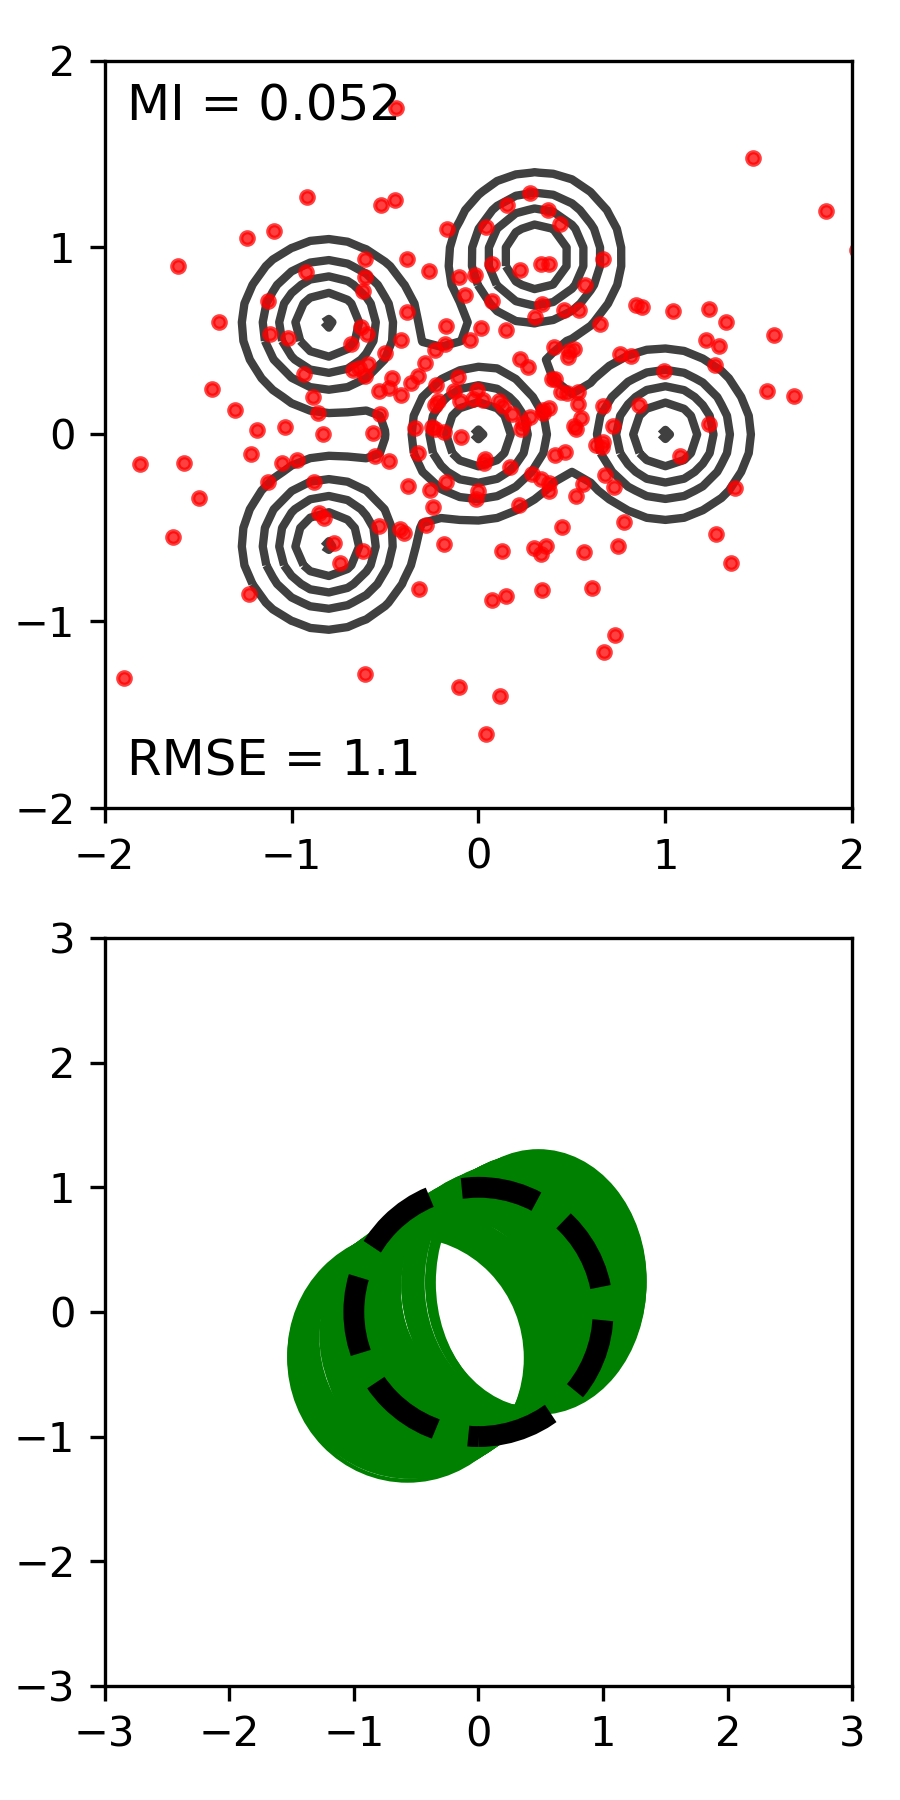
\includegraphics[width=0.165\columnwidth]{images/vae-as-mim-toy-2d/toy4/plots/vae_logvar10_mid-dim5_layers2_q-x0marginal_q-zx0_p-z0anchor_p-xz0/reconstruction_best.png}
    & 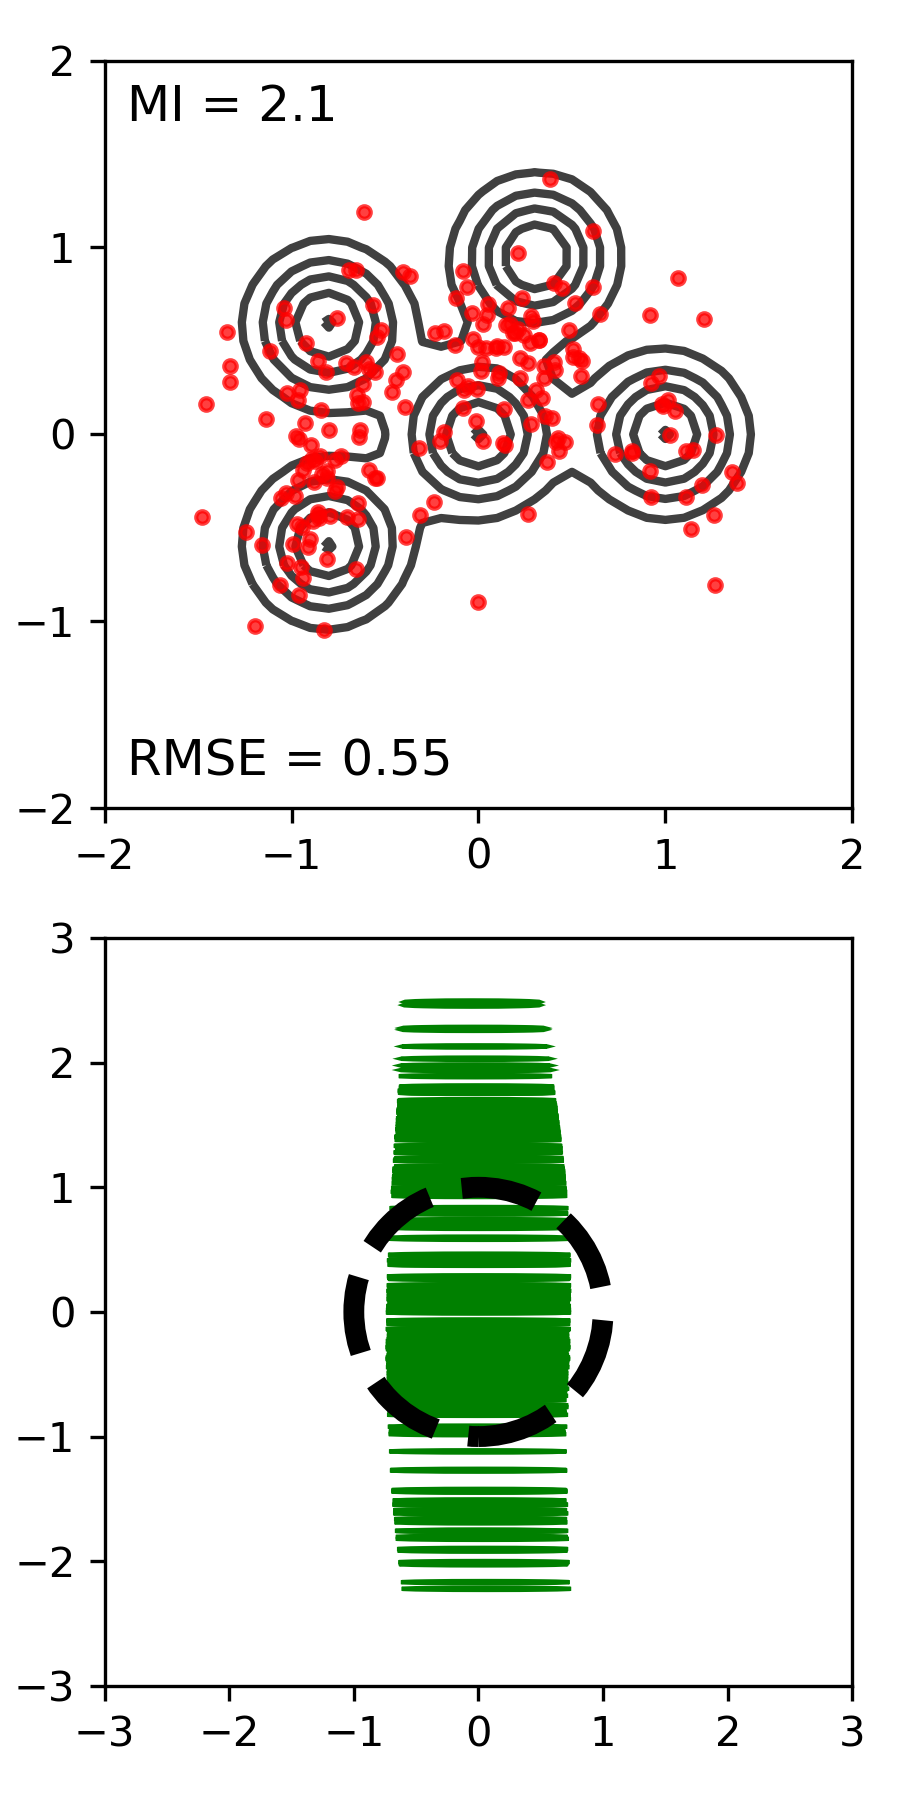
\includegraphics[width=0.165\columnwidth]{images/vae-as-mim-toy-2d/toy4/plots/mim-samp_logvar10_mid-dim5_layers2_q-x0marginal_q-zx0_p-z0anchor_p-xz0/reconstruction_best.png}
    & 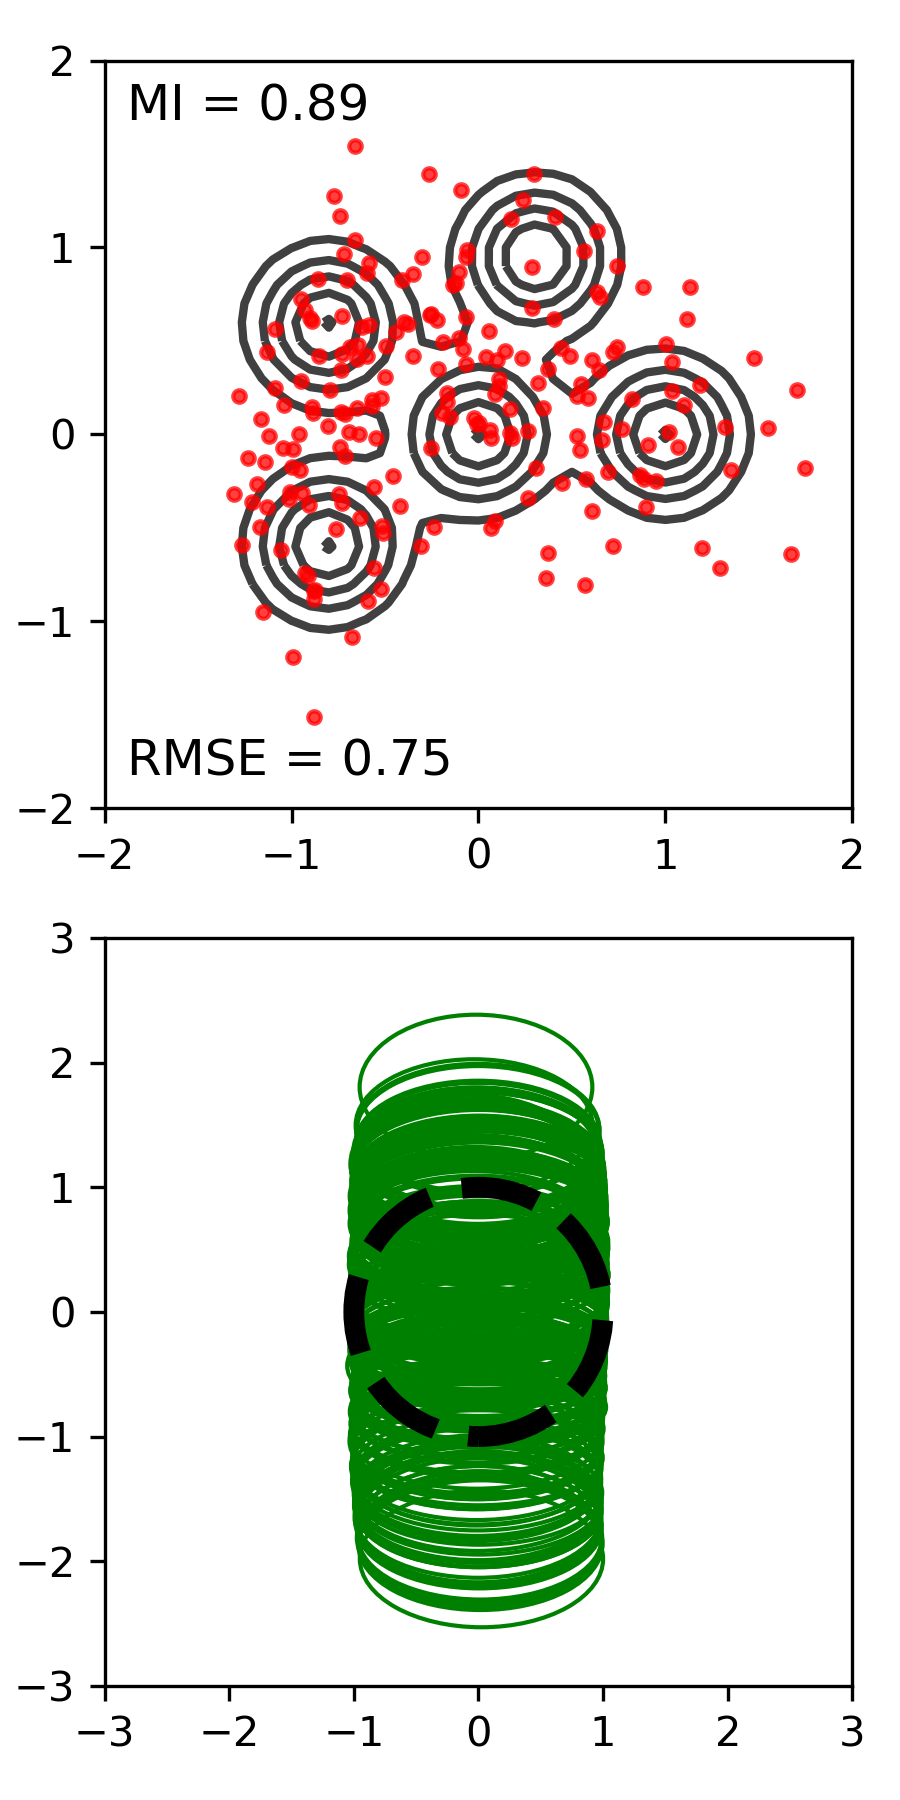
\includegraphics[width=0.165\columnwidth]{images/vae-as-mim-toy-2d/toy4/plots/vae_logvar10_mid-dim20_layers2_q-x0marginal_q-zx0_p-z0anchor_p-xz0/reconstruction_best.png}
    & 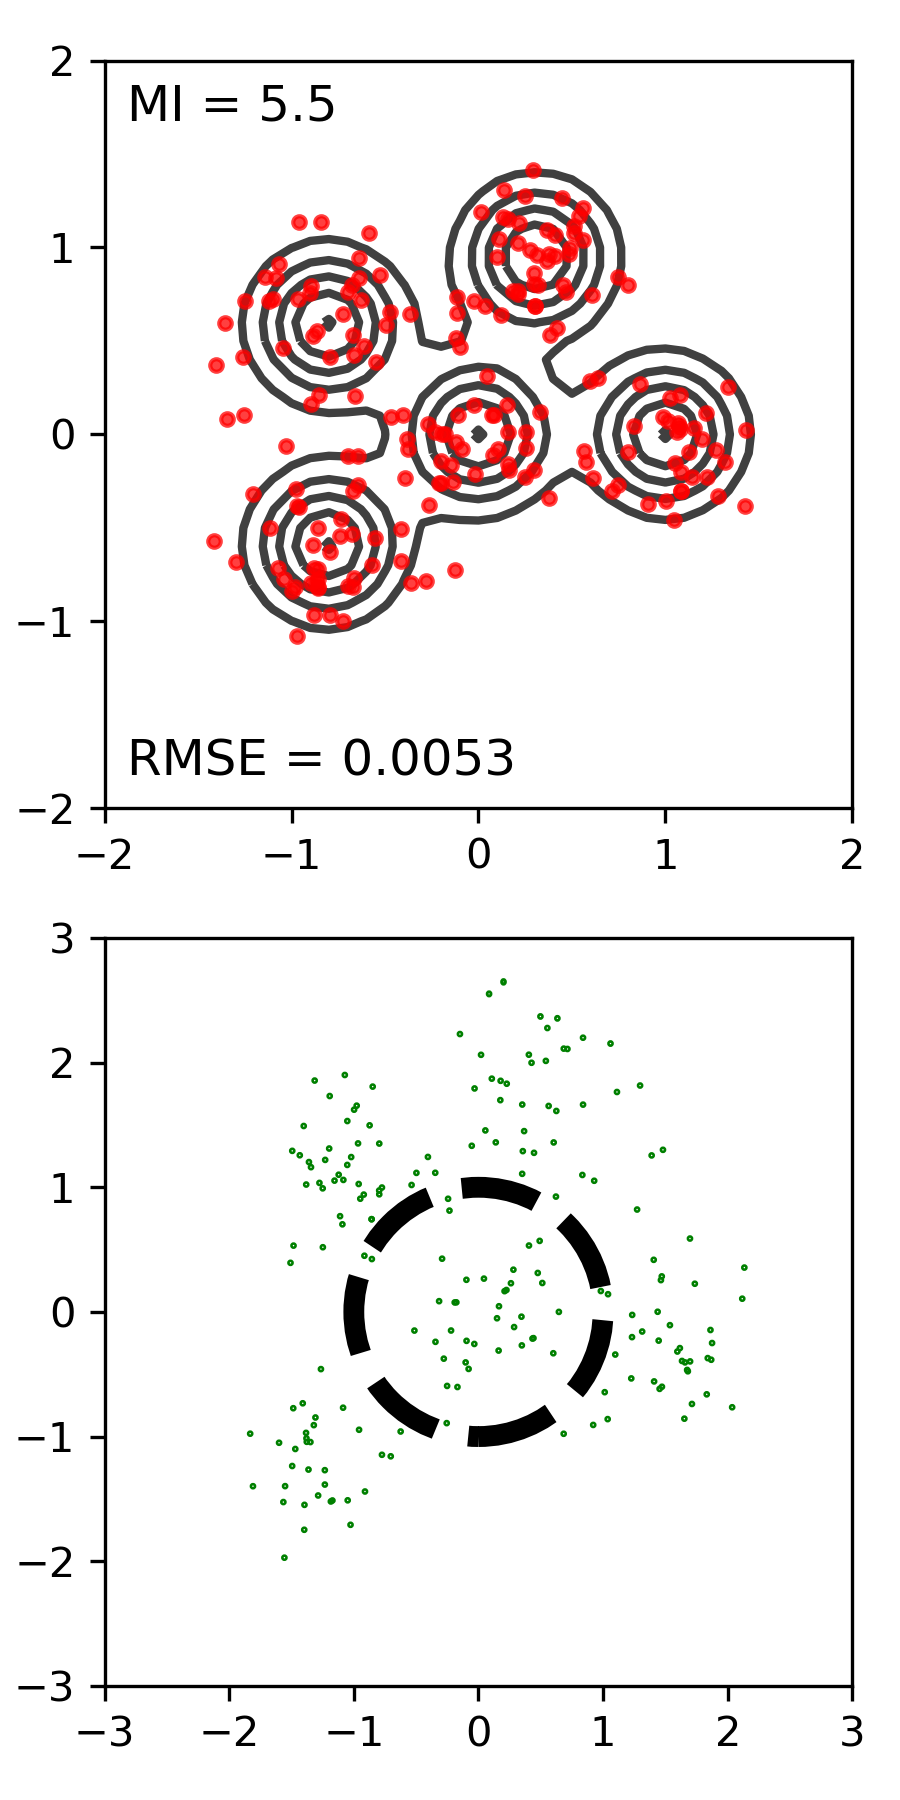
\includegraphics[width=0.165\columnwidth]{images/vae-as-mim-toy-2d/toy4/plots/mim-samp_logvar10_mid-dim20_layers2_q-x0marginal_q-zx0_p-z0anchor_p-xz0/reconstruction_best.png}
    & 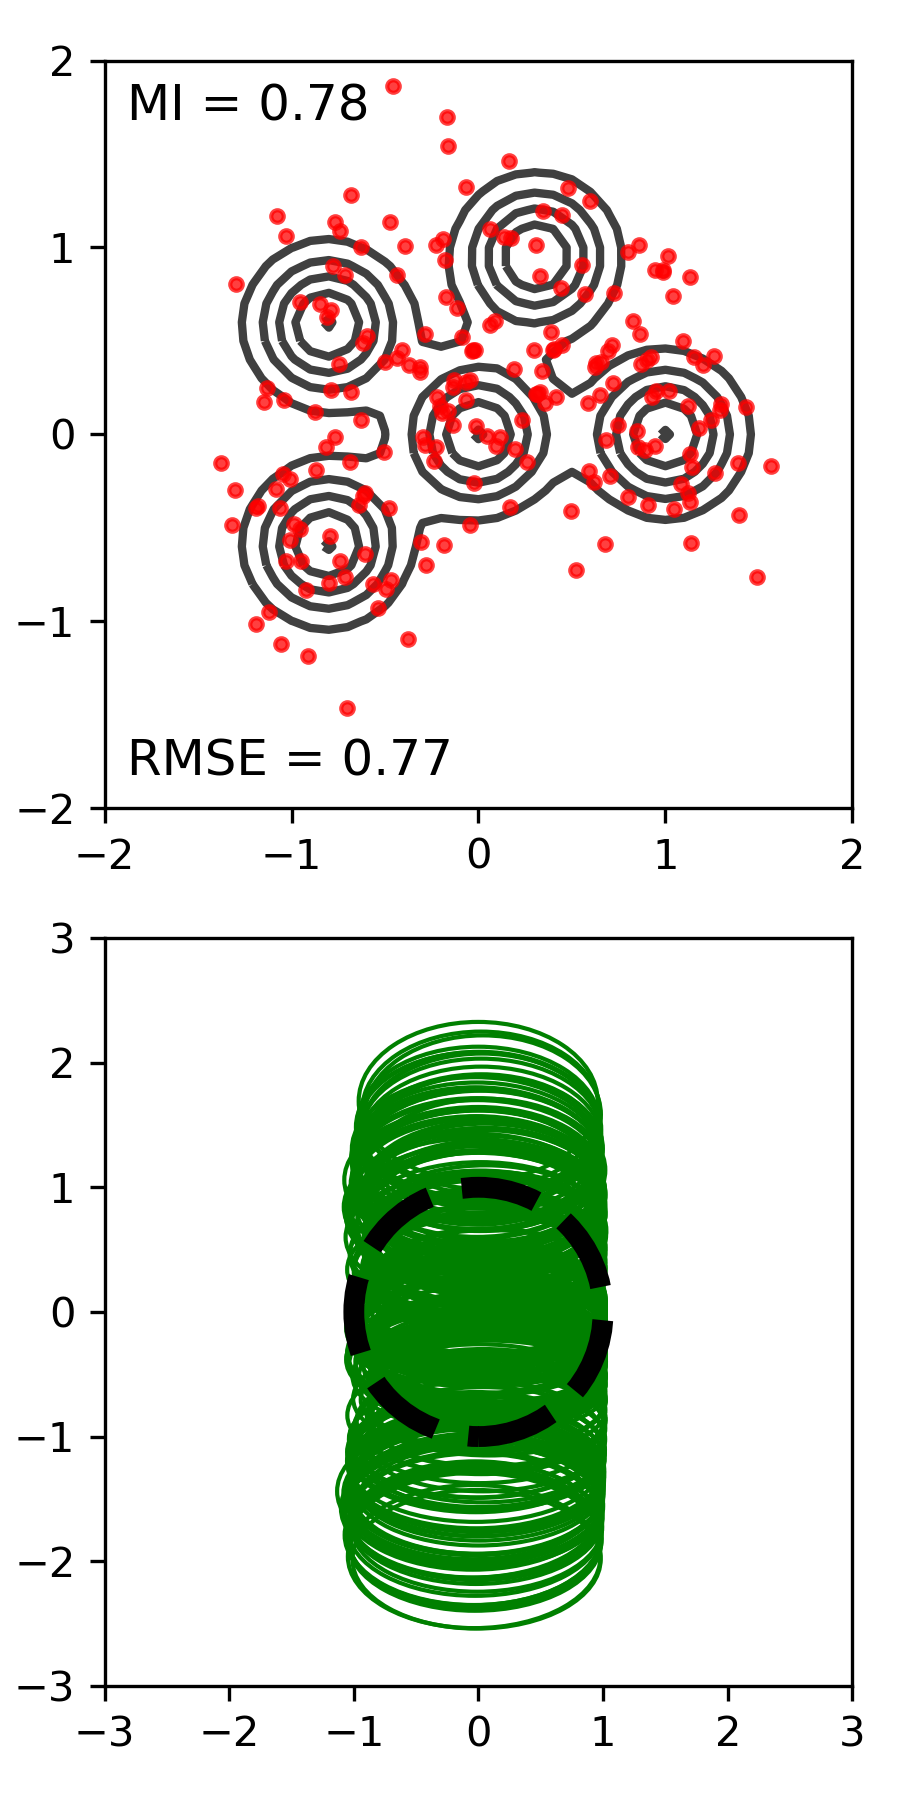
\includegraphics[width=0.165\columnwidth]{images/vae-as-mim-toy-2d/toy4/plots/vae_logvar10_mid-dim500_layers2_q-x0marginal_q-zx0_p-z0anchor_p-xz0/reconstruction_best.png}
    & 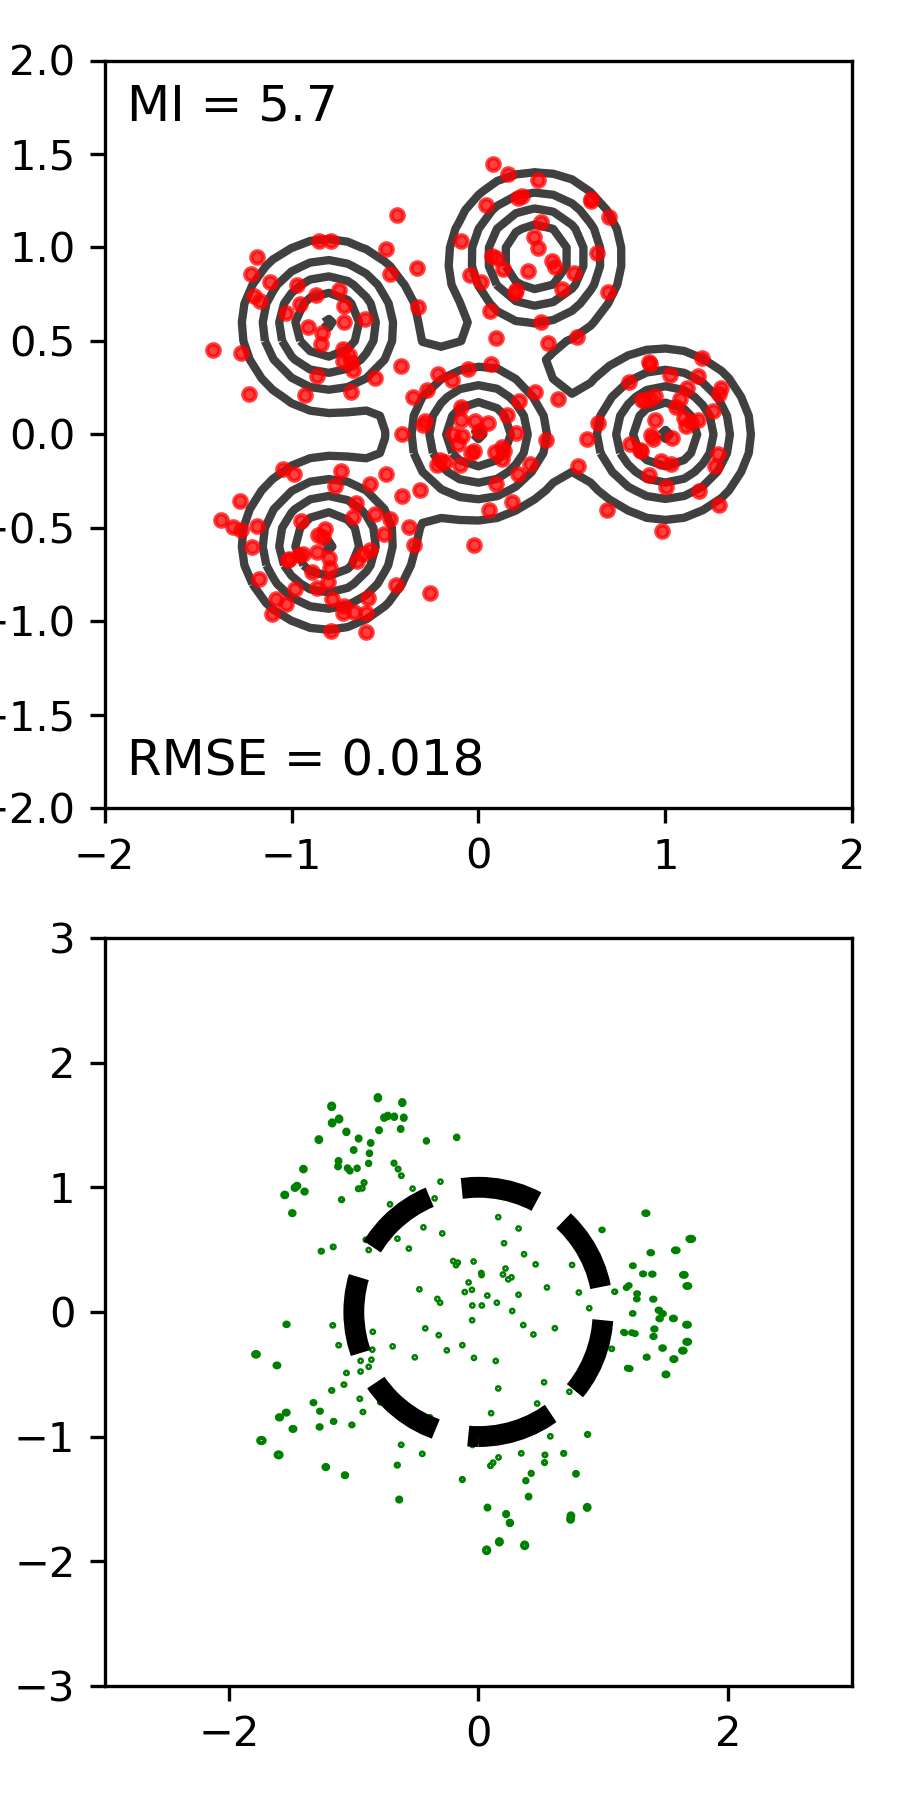
\includegraphics[width=0.165\columnwidth]{images/vae-as-mim-toy-2d/toy4/plots/mim-samp_logvar10_mid-dim500_layers2_q-x0marginal_q-zx0_p-z0anchor_p-xz0/reconstruction_best.png}
    \\
    \multicolumn{2}{c}{(a) $h \in \mathbb{R}^{5}$ } & \multicolumn{2}{c}{(b) $h \in \mathbb{R}^{20}$ } & \multicolumn{2}{c}{(c) $h \in \mathbb{R}^{500}$ } \\
    \end{tabular}
    \caption{
    VAE and MIM models with 2D inputs, a 2D latent space, and 5, 20 and 500 hidden units. 
    Top row: Black contours depict level sets of $\pjoint(\x)$, red points are 
    reconstructed test points.
    Bottom row: Green contours are one standard deviation ellipses of 
    $\Menc(\z|\x)$ for test points. Dashed black circles depict one standard 
    deviation of $\pjoint (\z)$.
    (a) For weak architectures MIM and VAE exhibit high posterior variance.
    (b,c) For more expressive architectures the VAE predictive variance remains high,
    an indication of posterior collapse.
    MIM generally produces lower predictive variance and lower reconstruction 
    errors, consistent with high mutual information (see inset quantities).
    }\label{fig:posterior-collapse-qualitative}
\end{figure}

\begin{figure}[ht]
    \centering
    \setlength{\tabcolsep}{0pt}
    \begin{tabular}{*4{>{\centering\arraybackslash}m{0.25\textwidth}}}
      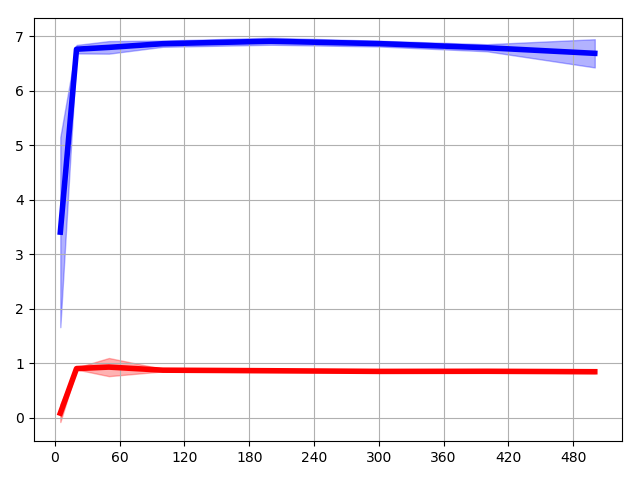
\includegraphics[width=0.24\columnwidth]{{images/vae-as-mim-toy-2d/toy4/stats/fig.MI_ksg}.png}
    & 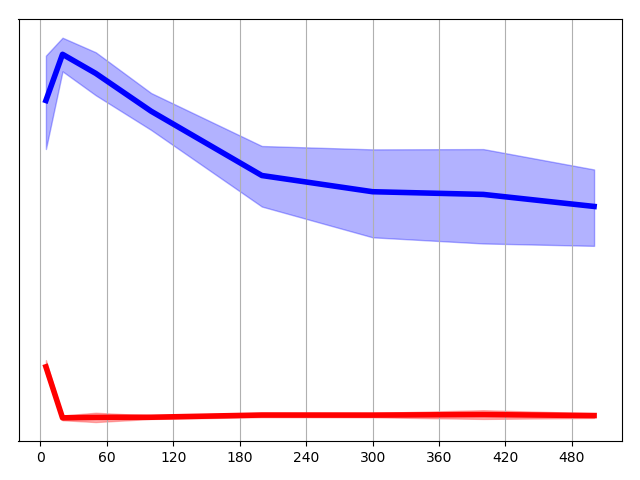
\includegraphics[width=0.24\columnwidth]{{images/vae-as-mim-toy-2d/toy4/stats/fig.H_q_x.symlog}.png}
    & 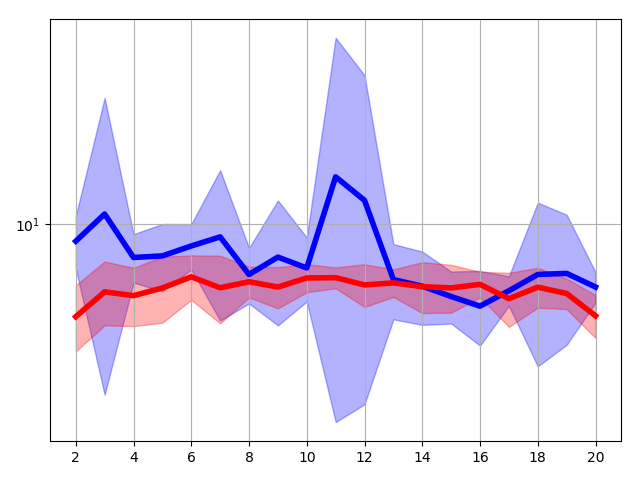
\includegraphics[width=0.24\columnwidth]{{images/vae-as-mim-toy-2d/toy4/stats/fig.x_recon_err.symlog}.png}
    & 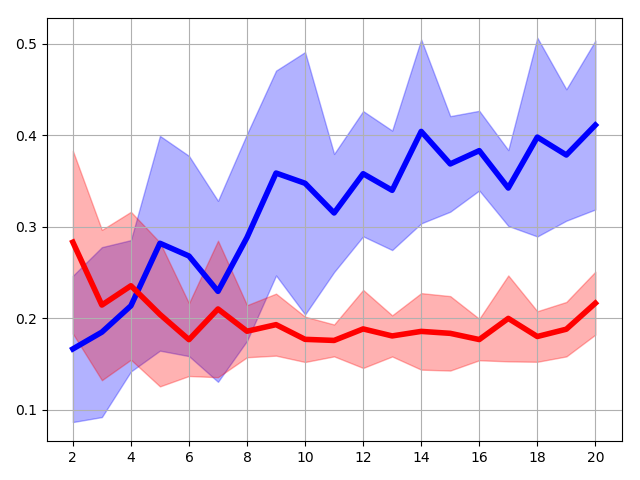
\includegraphics[width=0.24\columnwidth]{{images/vae-as-mim-toy-2d/toy4/stats/fig.clf_acc_KNN5}.png}
    \\
    (a) MI & (b)  $\E{\x \sim \pjoint(\x)}{\log \Menc(\x)}$ & (c) Recon.\ Error & (d) Classif.\ (5-NN)
    \end{tabular}
    \caption{Test performance for MIM (blue) and VAE (red) for 2D GMM experiment,
    all as functions of the number of hidden units (on x-axis), based on 10 learned
    models in each case. From left to right, plots show mutual information, log marginal 
    probability of test points, reconstruction error, and k-NN classification performance.
    \david{for these plots: link dots with lines, and on x-axis perhaps only label 20, 100, 
    200, 300, 400, and 500. Simpler format. Stdev bars or min-max?}\micha{will do. stdev in all plots}
    }\label{fig:posterior-collapse-quantitative}
\end{figure}


Bottom row of Fig.\ \ref{fig:posterior-collapse-qualitative}
depict the latent space behavior.  The dashed black circle 
depicts one standard deviation of $\pjoint(\z)$. Each green 
curve depicts a one standard deviation ellipse of the encoder posterior  
$\Menc(\z' | \x')$ for a data point $\x'$ drawn from $\pjoint(\x)$.
One can clearly see that for the weakest architecture, with only 5 
hidden units, both MIM and VAE posteriors have large variances.
When the number of hidden units increases to 20, however, it is 
clear that will the VAE posterior variance remains very large in
one dimension, the MIM encoder produces much tighter posteriors 
densities.  Even with more a expressive architecture, VAE posteriors depict
continue to exhibit very high variances, a common sign of posterior collapse. 



To quantify this behavior for each architecture in  
Fig.\ \ref{fig:posterior-collapse-qualitative}, Fig.\ 
\ref{fig:posterior-collapse-quantitative} plots the mutual information, 
the average log marginal of test points under the model $\Menc$,
the reconstruction error of test points, and 5-NN classification
(predicting which of five GMM components the test points were drawn from).
Following  \cite{Hjelm2018}, we estimate mutual information 
using the KSG mutual information estimator \cite{PhysRevE.69.066138,DBLP:journals/corr/GaoOV16},  
based on a K-NN neighborhoods with $k=5$, and measure the quality of the representation with classification axuliary task.

One can see that mutual information and the average log likelihood 
of the test data under the MIM model are higher than for VAE models.
One can also see that mutual information saturates for MIM as the
number of hidden units grow larger than 20.
(We direct the reader to Sec.\ \ref{sec:entropy-as-mi-regularizer}
of the supplementary material for experiments on variants of 
MIM and VAE tease apart the impact of specific terms of the 
respective objectives.)

One can also see from Fig.\ \ref{fig:posterior-collapse-qualitative} that as the models 
becomes sufficiently expressive, in terms of the number of 
hidden units, the MIM encoding variance becomes extremely small,
and the reconstruction error in Fig.\ \ref{fig:posterior-collapse-quantitative} approaches 0.
Effectively, the encoder and decoder learn an (approximately) invertible mapping using 
an unconstrained architecture (demonstrated here for the 2D case), when the 
dimensionality of the latent representation and the observations is the same.

The VAE, by comparison, is prone to posterior collapse, with latent embeddings 
with relatively low mutual information. In regard, we note that several 
papers have described ways to mitigate posterior collapse in VAE learning, e.g., 
by lower bounding, or annealing the KL divergence term in the VAE objective 
(e.g., \citep{DBLP:journals/corr/abs-1711-00464,DBLP:journals/corr/abs-1901-03416}), 
or by limiting the expressiveness of the decoder (e.g., \citep{ChenKSDDSSA16}).
We posit that MIM does not suffer from this problem as a consequence of 
the objective design principles that encourage high mutual information
between observations and the latent representation.


\bibliographystyle{plainnat}
\bibliography{paper}

\end{document}
